%******************************************************************************%
% Copyright (C) 2018  Louis Solofrizzo                                         %
%                                                                              %
% This content is considered a free software: you can redistribute it          %
% and/or modify it under the terms of the GNU General Public License as        %
% published by the Free Software Foundation, either version 3 of the License,  %
% or (at your option) any later version.                                       %
%                                                                              %
% This program is distributed in the hope that it will be useful,              %
% but WITHOUT ANY WARRANTY; without even the implied warranty of               %
% MERCHANTABILITY or FITNESS FOR A PARTICULAR PURPOSE.  See the                %
% GNU General Public License for more details.                                 %
%                                                                              %
% You should have received a copy of the GNU General Public License            %
% along with this program.  If not, see <https://www.gnu.org/licenses/>.       %
%******************************************************************************%

%******************************************************************************%
%                                                                              %
%                          KFS_7.en.tex for KFS_7                              %
%                                                                              %
%                  Created on : Wed May 25 13:27:28 2016                       %
%          Made by : Louis "Ne02ptzero" Solofrizzo <louis@ne02ptzero.me>       %
%                                                                              %
%******************************************************************************%

\documentclass{42-en}

%******************************************************************************%
%                                                                              %
%                                    Header                                    %
%                                                                              %
%******************************************************************************%
\begin{document}

                           \title{KFS\_7}
                          \subtitle{Syscalls, Sockets and env}
                       \member{Louis Solofrizzo}{louis@ne02ptzero.me}
                        \member{42 Staff}{pedago@42.fr}

\summary {
    The real stuff.
}

\maketitle

\tableofcontents

%******************************************************************************%
%                                                                              %
%                                  Foreword                                    %
%                                                                              %
%******************************************************************************%
\chapter{Foreword}
    \subsection{A developer's life in a nutshell}
    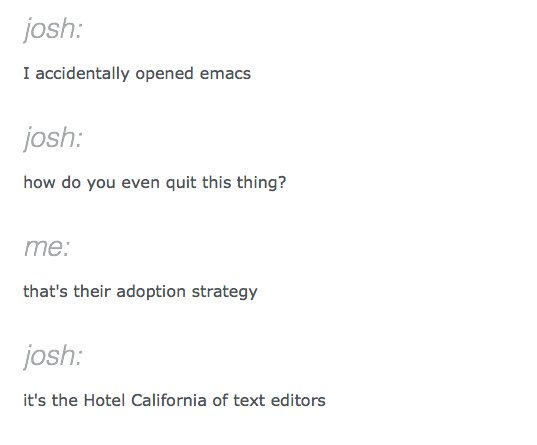
\includegraphics[width=8cm]{./1.jpeg}
    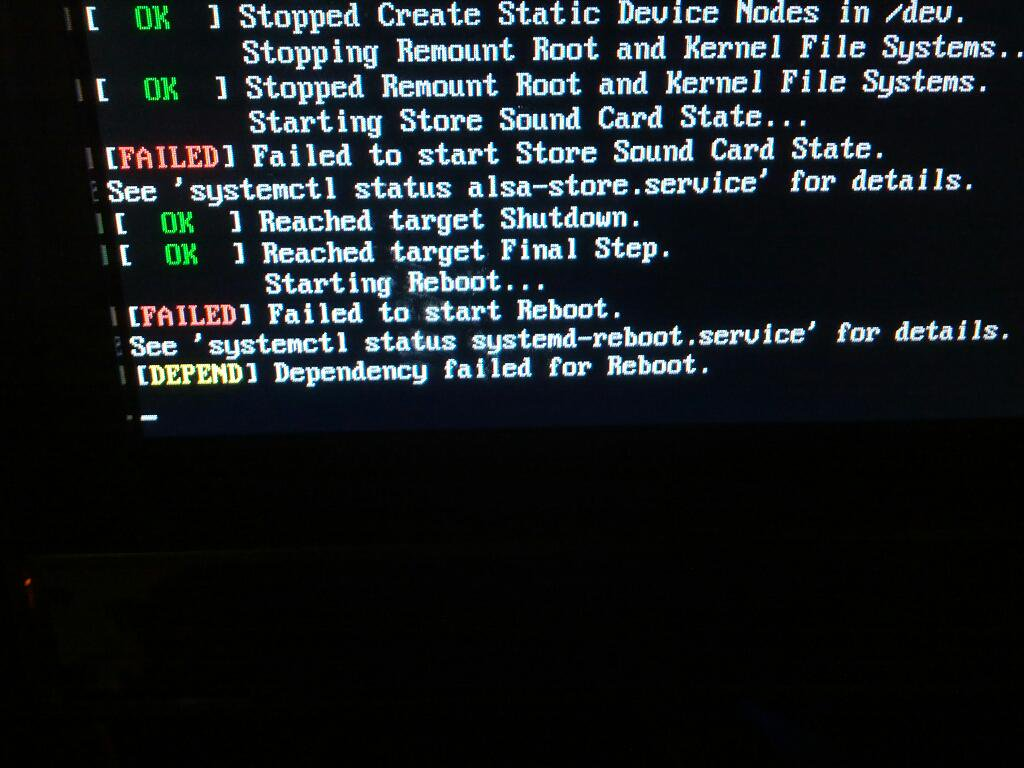
\includegraphics[width=9cm]{./2.jpeg}
    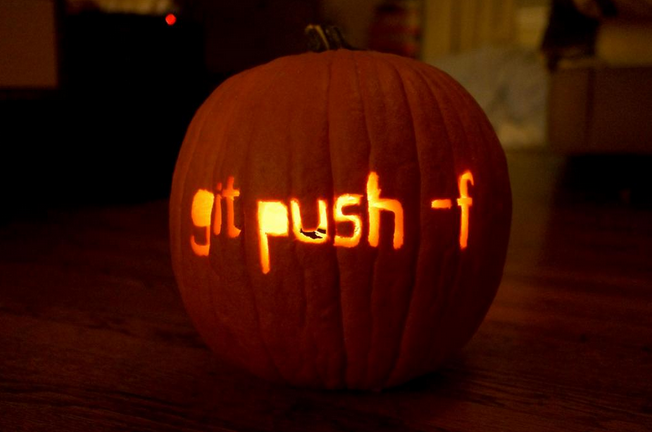
\includegraphics[width=8cm]{./3.png}
    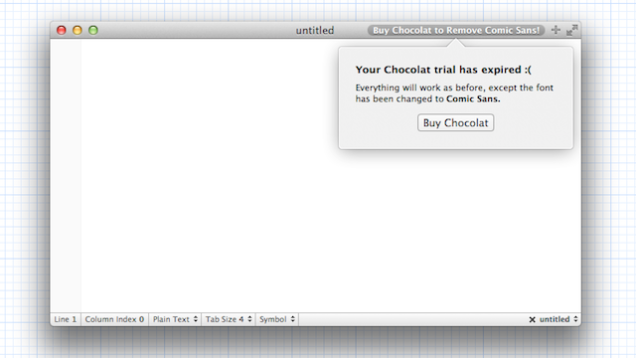
\includegraphics[width=9cm]{./4.png}

%******************************************************************************%
%                                                                              %
%                                 Introduction                                 %
%                                                                              %
%******************************************************************************%
\chapter{Introduction}
    \subsection{Syscalls}
        \begin{quotation}
            \textit{In computing, a system call is the programmatic way in
            which a computer program requests a service from the kernel of the
            operating system it is executed on. This may include
            hardware-related services (for example, accessing a hard disk
            drive), creation and execution of new processes, and communication
            with integral kernel services such as process scheduling. System
            calls provide an essential interface between a process and the
            operating system.}
        \end{quotation}
        It's time to implement syscalls, and code them! Sounds fun, eh?
        Syscalls are stored in a \texttt{Syscall table}, in order to keep the
        Kernel code clean. You can look at the one on Linux if you don't know
        anything about \texttt{Syscall tables}. Now let's talk about the
        runtime. When a process (usually a user-space process) calls a syscall,
        a standard function is called (wrapper) and calls in turn the kernel
        with the number of the said syscall. Here is a pratical example:\\
        \begin{itemize}\itemsep1pt
            \item In my a.out, I call the syscall \texttt{write}.
            \item The wrapper in \texttt{unistd.h} calls a
            \texttt{do\_syscall(int n, ...)} function in order to tell the
            kernel that this process wants to use this function.
        \end{itemize}
        Now there is a design problem. As you know, the kernel cannot
        directly interact with user space, that's the role of syscalls!
        So, how can a syscall get to the kernel? The answer's pretty simple:
        the \texttt{IDT}. Let's see our simple example again:
        \begin{itemize}\itemsep1pt
            \item The \texttt{do\_syscall} function calls an ASM function that
            calls your kernel function.
            \item For that to happen, you must configure the IDT so that it
            listens to \texttt{0x30}, and calls your ASM function.
        \end{itemize}
        And that's it. It's actually a pretty simple process - with a well
        designed kernel.
\newpage
    \subsection{Environment}
        I'm sure you all know how a \texttt{Unix Environment} works, but let's
        do a quick recap:
        \begin{itemize}\itemsep1pt
            \item The Environment is composed of variables with a name, and a
            value.
            \item These variables can be modified, deleted, and a new variable
            can be added too.
            \item When a process is created, the father process' environment
            is passed as a third argument in the main function.
            \item If the process is the master (first process after the Kernel,
            or launched by the kernel itself) a default environment is set.
            \item When the child process is exited, the father environment is
            not affected.
            \item Multiple processes can have different environments.
        \end{itemize}
    \subsection{User accounts}
        In a Unix system, a user account is a user that has the following
        attributes:
        \begin{itemize}\itemsep1pt
            \item A user name.
            \item A user identifier (UID).
            \item A group identifier (GID).
            \item A home's directory.
            \item A program that is launched at every login.
        \end{itemize}
        If you're familiar with Linux, you'll have guessed that I just described
        the \texttt{/etc/passwd} file. Nothing too complex here either, just a
        basic code structure with stored data.
    \subsection{Password protection}
        In modern Unix systems, the OS will only deal with hashed passwords
        in order to protect the system. In Linux, those hashes are stored in
        \texttt{/etc/shadow}. Here's the wikipedia definition:
        \begin{quotation}
            \textit{/etc/shadow is used to increase the security level of
            passwords by restricting all but highly privileged users' access to
            hashed password data. Typically, that data is kept in files owned
            by and accessible only by the super user.
            Systems administrators can reduce the likelihood of brute force
            attacks by making the list of hashed passwords unreadable by
            unprivileged users. The obvious way to do this is to make the
            passwd database itself readable only by the root user. However,
            this would restrict access to other data in the file such as
            username-to-userid mappings, which would break many existing
            utilities and provisions. One solution is a "shadow" password file
            to hold the password hashes separate from the other data in the
            world-readable passwd file. For local files, this is usually
            /etc/shadow on Linux and Unix systems, or /etc/master.passwd on BSD
            systems; each is readable only by root. (Root access to the data is
            considered acceptable since on systems with the traditional
            "all-powerful root" security model, the root user would be able to
            obtain the information in other ways in any case). Virtually all
            recent Unix-like operating systems use shadowed passwords.}
        \end{quotation}
    \newpage
    \subsection{Inter-Process Communication Socket}
        \begin{quotation}
            \textit{A Unix domain socket or IPC socket (inter-process
            communication socket) is a data communications endpoint for
            exchanging data between processes executing on the same host
            operating system. Like named pipes, Unix domain sockets support
            transmission of a reliable stream of bytes (SOCK\_STREAM, compare to
            TCP). In addition, they support ordered and reliable transmission
            of datagrams (SOCK\_SEQPACKET), or unordered and unreliable
            transmission of datagrams (SOCK\_DGRAM, compare to UDP). The Unix
            domain socket facility is a standard component of POSIX operating
            systems.}
        \end{quotation}
        Besides network uses, a socket is mainly used for inter-process
        communication. Usually, the syscalls \texttt{sendmsg()} and
        \texttt{recvmsg()} are used for that. In a Unix system, a socket is a
        file, with a file descriptor shared between the two communicating
        processes.
    \subsection{Filesystem Hierarchy}
        As you may know, in a Unix system, everything is a file. Like
        \texttt{/dev/sda} is a hard drive, and \texttt{/dev/sda1} is a
        partition. And the \texttt{/proc} folder contains all the processes of
        the kernel. There are many examples for this rule, I invite you to
        look it up by yourself.

%******************************************************************************%
%                                                                              %
%                                  Goals                                       %
%                                                                              %
%******************************************************************************%
\chapter{Goals}

    At the end of this project, you will have:
    \begin{itemize}\itemsep1pt
        \item A complete syscall table with a syscall system.
        \item A complete Unix Environment.
        \item User accounts, with login and password.
        \item Password protection.
        \item Inter-Process Communication socket.
        \item A Unix-like filesystem Hierarchy.
    \end{itemize}

%******************************************************************************%
%                                                                              %
%                             General instructions                             %
%                                                                              %
%******************************************************************************%
\chapter{General instructions}
    \section{Code and Execution}
        \subsection{Emulation}
        The following part is not mandatory, you're free to use any virtual
        manager you want; however, I suggest you use \texttt{KVM}.
        It's a \texttt{Kernel Virtual Manager} with advanced execution
        and debug functions.
        All of the examples below will use \texttt{KVM}.
        \subsection{Language}
            The \texttt{C} language is not mandatory, you can use any language
            you want for this series of projects.\\
            Keep in mind that not all languages are kernel friendly, you could
            code a kernel in \texttt{Javascript}, but are you sure it's a
            good idea?\\
            Also, most of the documentation is written in \texttt{C}, you will
            have to 'translate' the code all along if you choose a different
            language.\\

            Furthermore, not all the features of a given language can be used
            in a basic kernel. Let's take an example with \texttt{C++}:\\
            this language uses 'new' to make allocations, classes and
            structures declarations. But in your kernel you don't have a memory
            interface (yet), so you can't use any of these features.\\

            Many languages can be used instead of \texttt{C},
            like \texttt{C++}, \texttt{Rust}, \texttt{Go}, etc.
            You can even code your entire kernel in \texttt{ASM}!\\
            \begin{center}
              
\includegraphics[width=8cm]{choose.jpg}
            \end{center}
\newpage

    \section{Compilation}
        \subsection{Compilers}
            You can choose any compiler you want. I personaly use \texttt{gcc}
            and \texttt{nasm}. A Makefile must be turned-in as well.
        \subsection{Flags}
            In order to boot your kernel without any dependency, you must
            compile your code with the following flags (adapt the flags for
            your language, these are \texttt{C++} examples):
            \begin{itemize}\itemsep1pt
                \item \texttt{-fno-builtin}
                \item \texttt{-fno-exception}
                \item \texttt{-fno-stack-protector}
                \item \texttt{-fno-rtti}
                \item \texttt{-nostdlib}
                \item \texttt{-nodefaultlibs}
            \end{itemize}
            You might have noticed these two flags: \texttt{-nodefaultlibs}
            and \texttt{-nostdlib}. Your Kernel will be compiled on a host
            system, that's true, but it cannot be linked to any existing
            library on that host, otherwise it will not be executed.
    \section{Linking}
        You cannot use an existing linker in order to link your kernel.
        As mentionned above, your kernel would not be initialized. So you must
        create a linker for your kernel.\\
        Be careful, you \texttt{CAN} use the 'ld' binary available on your
        host, but you \texttt{CANNOT} use the .ld file of your host.
    \section{Architecture}
        The \texttt{i386} (x86) architecture is mandatory (you can thank
        me later).
    \section{Documentation}
        There is a lot of documentation available, good and bad.
        I personaly think the \texttt{\href{http://wiki.osdev.org/Main_Page}
        {OSDev}} wiki is one of the best.
    \section{Base code}
        In this subject, you have to take your previous \texttt{KFS} code,
        and work from it!\\
        Or don't. And rewrite everything from scratch. Your call!
\newpage

%******************************************************************************%
%                                                                              %
%                             Mandatory part                                   %
%                                                                              %
%******************************************************************************%
\chapter{Mandatory part}
%%- Mise a la norme POSIX pour tout le kernel
%- Implementation de la table des syscalls
%- Creation de l'env et de son interface
%- Creation des comptes utilisateurs
%Sockets UNIX pour communication inter-processus
%- Introduction du temps atomique et du temps lineaire
%- Liaison des peripheriques aux /dev correspondants (en particulier les TTY)

%- T3
%- Groupes de 2 a 3 etudiants
%- 4 semaines
    In this subject you will have to:
    \begin{itemize}\itemsep1pt
        \item Implement a functional and complete syscall interface:
        \begin{itemize}\itemsep1pt
            \item A syscall table.
            \item An ASM function for the IDT callback.
            \item A kernel-side function that takes the number of the syscall,
            gets the arguments of the call, places them in the register and pushes
            the call on the stack.
            \item You must proove that your code works by creating a process,
            have it use a syscall, and print the used syscall on the screen.
        \end{itemize}
        \item Implement a working unix environment. (cf. Intro)
        \item Users accounts, with password protection by obscurity. (cf. Intro)
        \item Inter-Process Sockets, working via syscalls, with shared file
        descriptors.
        \item Implement a complete file Hierarchy, Unix-like (cf. Intro).
    \end{itemize}
    All of these points must be checked thorougly during the peer-corrections,
    so write some debug in it to facilitate the process.

%******************************************************************************%
%                                                                              %
%                                 Bonus part                                   %
%                                                                              %
%******************************************************************************%
\chapter{Bonus part}
    Change your kernel console so that a user can use a console with their own
    environment, like a real OS.\\
    Implement different ttys, with the appropriate files in /dev.

%******************************************************************************%
%                                                                              %
%                           Turn-in and peer-evaluation                        %
%                                                                              %
%******************************************************************************%
\chapter{Turn-in and peer-evaluation}
    Turn your work in using your \texttt{GiT} repository, as
    usual. Only the work that's in your repository will be graded during
    the evaluation.

    Your must turn in your code, a Makefile and a basic virtual image for your kernel.\\
    Side note about this image,
    THERE IS NO NEED TO BE BUILT LIKE AN ELEPHANT.

%******************************************************************************%
\end{document}
